\documentclass{article}
\usepackage[spanish]{babel}
\usepackage[utf8]{inputenc}
\usepackage{graphicx}
\usepackage{minted}

\title{\textbf{Criptografía aplicada: Cálculo del hash SHA-256 de un bloque Bitcoin}}
\author{Javier Domínguez Gómez \\
\small{jdg@member.fsf.org} \\
\small{Fingerprint: 94AD 19F4 9005 EEB2 3384 C20F 5BDC C668 D664 8E2B}}
\date{v0.1.03 - Febrero 2019}

\usepackage{courier}
\begin{document}
\maketitle

\tableofcontents{}

\section{Introducción}
    Este documento describe en detalle las partes de la cabecera de un bloque cualquiera en la cadena de bloques de Bitcoin, así como las operaciones lógico-matemáticas de la función criptográfica SHA-256 que se emplean con el fin de generar el \textit{hash} adecuado que finalmente representará dicho bloque en la cadena de bloques.

\section{Estructura de datos de un bloque}
    \vspace{3mm}
    Cada bloque de la cadena de bloques de Bitcoin contiene una estructura de datos que se puede categorizar en la siguiente tabla.
    \begin{table}[H]
    \centering
    \begin{tabular}{| c | l | c | l |} 
        \hline
        Tipo de dato & Nombre & Tamaño & Formato \\
        \hline
        uint32\_t & magicID & 4 bytes & Little-endian \\
        \hline
        uint32\_t & headerLenght & 4 bytes & Big-endian \\
        \hline
        uint32\_t & versionNumber & 4 bytes & Little-endian \\
        \hline
        uint8\_t[32] & previousBlockHash & 32 bytes & Big-endian \\
        \hline
        uint8\_t[32] & merkleRoot & 32 bytes & Big-endian \\
        \hline
        uint32\_t & timeStamp & 4 bytes & Little-endian \\
        \hline
        uint32\_t & targetDifficulty & 4 bytes & Little-endian \\
        \hline
        uint32\_t & nonce & 4 bytes & Little-endian \\
        \hline
        uint8/16/32/64\_t & transactionCount & 1, 3, 5 o 9 bytes & Big-endian*  \\
        \hline
    \end{tabular}
    \caption{Datos de la cabecera de un bloque en la cadena de bloques de Bitcoin.}
    \label{table:0}
    \end{table}
    
    *En el caso de \textit{transactionCount}, los enteros grandes se codifican en formato \textit{Little-endian}.
    
    \subsection{magicID}
    Se trata de un dato de 4 bytes de longitud. Se establece como prefijo en cada uno de los mensajes entre los nodos para identificar la red de Bitcoin en la que se generan. La siguiente tabla muestra los diferentes valores que puede tener la variable magicID dependiendo de la red.
    
    \begin{table}[H]
    \centering
    \begin{tabular}{| c | c |} 
        \hline
        Red & magicID \\
        \hline
        Mainnet & \texttt{0xf9beb4d9} \\
        \hline
        Testnet & \texttt{0xfabfb5da} \\
        \hline
        Testnet3 & \texttt{0x0b110907} \\
        \hline
        Namecoin & \texttt{0xf9beb4fe} \\
        \hline
        Regtest & \texttt{0xfabfb5da} \\
        \hline
    \end{tabular}
    \label{table:1}
    \end{table}
    
    No solo sirve como dato identificativo de una red en particular, también cumple la función de delimitador entre mensajes y entre los datos de cada bloque, pues estos vienen concatenados en cadenas hexadecimales uno a continuación de otro.
    
    Se decidió establecer estos valores tan específicos dada la improbabilidad de que los caracteres ASCII que representan se encuentren en un mensaje estándar, tal y como se indica en el archivo \textit{chainparams.cpp}\footnote{https://github.com/bitcoin/bitcoin/blob/master/src/chainparams.cpp\#L99} que lo implementa en el código de Bitcoin.
    
    \subsection{headerLenght}
    Este dato representa la longitud en bytes del bloque actual.
    
    \subsection{versionNumber}
    Este dato puede cambiar de valor cuando se actualiza el software y cambia el número de la versión del protocolo. El valor actual es 0x02000000 y se codifica en formato \textit{Little-endian}.
    
    \subsection{previousBlockHash}
    Se trata del \textit{hash} o \textit{digest} resultante del bloque anterior tras aplicar las funciones criptográficas utilizando los datos de la cabecera de dicho bloque. Tiene una longitud de 256 bits o 32 bytes codificado en formato \textit{Big-endian}.
    
    \subsection{merkleRoot}
    Este dato se modifica cada vez que una nueva transacción es aceptada. Tiene una longitud de 256 bits o 32 bytes codificado en formato \textit{Big-endian}
    
    \begin{figure}[H]
    \centering
        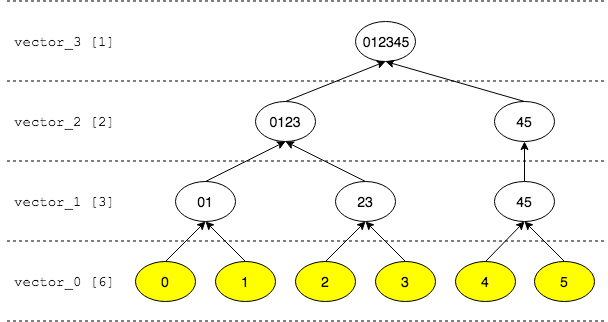
\includegraphics[scale=0.55]{img/Merkle_tree_05_leaves_nodes}
        \caption{Ejemplo de árbol de Merkle con 5 nodos hoja}
    \end{figure}
    
    \subsection{timeStamp}
    Se trata de un dato de 4 bytes de longitud en un formato numérico llamado Epoch o Tiempo Unix. Representa el número de segundos que han transcurrido desde el 1 de enero de 1970 a las 00:00. Se codifica en formato \textit{Little-endian}.
    
        \subsubsection{Fecha en formato Unix}
        \begin{figure}[H]
        \centering
            \begin{minted}{c}
        #include <stdio.h>
        #include <time.h>
        
        int main(int argc, char *argv[]) {
        
        	int year, month, day, hour, minute, second;
        	struct tm t;
        	time_t tod;
        
        	printf("Year: ");
        	scanf("%d", &year);
        	printf("Month: ");
        	scanf("%d", &month);
        	printf("Day: ");
        	scanf("%d", &day);
        	printf("Hour: ");
        	scanf("%d", &hour);
        	printf("Minute: ");
        	scanf("%d", &minute);
        	printf("Second: ");
        	scanf("%d", &second);
        
        	t.tm_year = year - 1900;
        	t.tm_mon = month - 1;   // Values [0-11]
        	t.tm_mday = day;
        	t.tm_hour = hour + 1;   // GMT+1
        	t.tm_min = minute;
        	t.tm_sec = second;
        	t.tm_isdst = 0;         // DST = 0
        	tod = mktime(&t);
        
        	printf("Timestamp epoch: %ld\n", (long) tod);
        }
            \end{minted}
        \end{figure}
    
    \subsection{targetDifficulty}
    Se trata de un número de 256 bits representado como un número decimal muy grande, tanto que abarcaría el rango de números que existen entre $0$ y $2^{256}-1$. Su función es la de definir una variable más a tener en cuenta a la hora de obtener el hash adecuado de un bloque antes de ser minado. Así pues la prueba de trabajo o \textit{Proof of Work} tendrá mayor o menor dificultad. En el protocolo de Bitcoin se define una regla que dice que el \textit{hash} del bloque ha de ser un número menor o igual al valor de la variable \textit{targetDifficulty} en ese momento. Así pues, si el \textit{hash} obtenido como candidato a generar un bloque fuera un número menor o igual al de \textit{targetDifficulty} habría posibilidades para que el hash candidato sea un \textit{hash} válido para generar un nuevo bloque, aunque de forma adicional se han de cumplir otras condiciones. Por el contrario, si el \textit{hash} obtenido como candidato fuera un número mayor que el valor de la variable \textit{targetDifficulty}, en ese caso se ha de incrementar el valor de la variable \textit{nonce} y probar otra vez a generar un \textit{hash} nuevo.
    
    \begin{figure}[H]
    \centering
        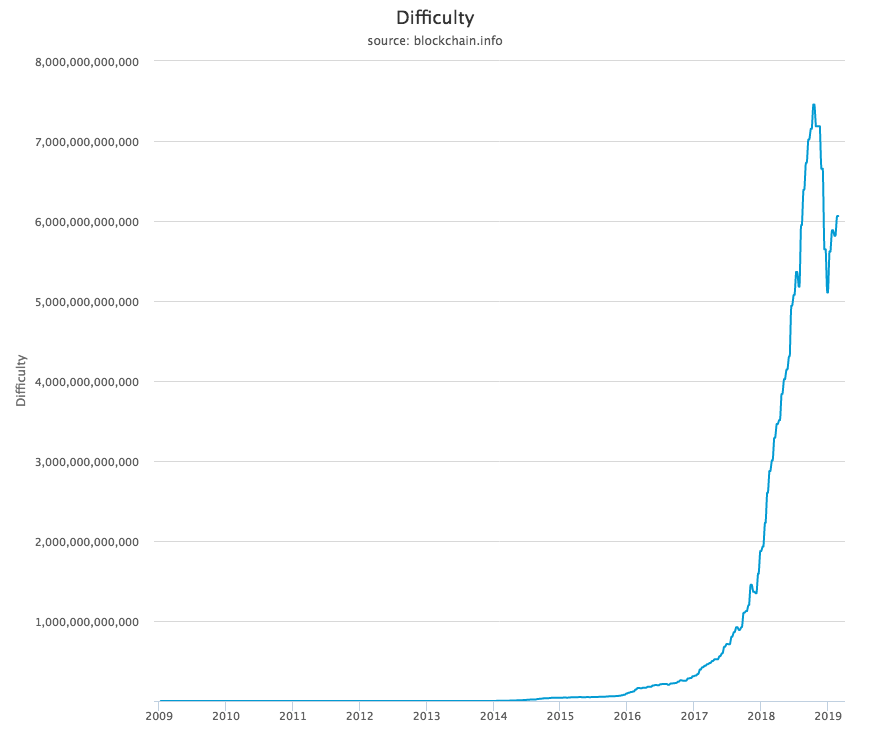
\includegraphics[scale=0.39]{img/Bitcoin_TargetDifficulty.png}
        \caption{Valor de la variable \textit{targetDifficulty} desde enero de 2009 hasta hoy.}
    \end{figure}
    
    El valor de la variable \textit{targetDifficulty} se modifica automáticamente una vez se han generado 2016 bloques, esto sucede aproximadamente cada dos semanas. El nuevo valor se obtiene mediante un cálculo que realizan todos los clientes Bitcoin de la red en el que toman el tiempo real que ha llevado generar los 2016 bloques y se obtiene la diferencia porcentual respecto al número de bloques que se esperaba haber calculado en el periodo de dos semanas.
    
    \subsection{nonce}
    Se trata de un número aleatorio con una longitud de 32 bits codificado en formato \textit{Little-endian}.
    
    \subsection{transactionCount}
    En el caso de transactionCount el tipo de dato es un \textit{entero de longitud variable}\footnote{https://en.bitcoin.it/wiki/Protocol\_documentation\#Variable\_length\_integer}.
    
    \begin{figure}[H]
    \centering
        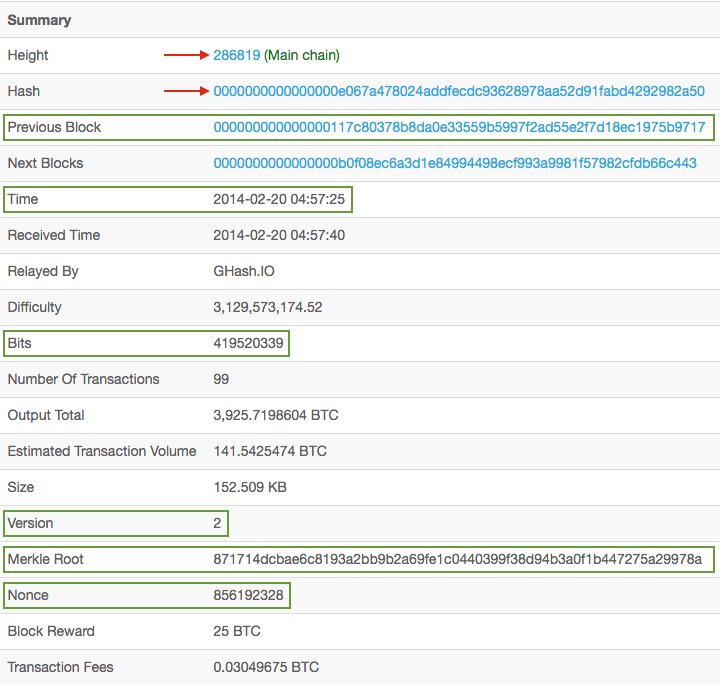
\includegraphics[scale=0.47]{img/Bitcoin_block_SHA_256_Block_Data}
        \caption{Datos empleados para la obtención del \textit{hash} del bloque $286819$.}
    \end{figure}
    
    \vspace{3mm}
    En la siguiente figura se detalla el contenido de los primeros 16 registros de la variable $W_{t}$ en cada una de las tres veces que se ejecutan las 64 iteraciones de la función SHA-256 para obtener el \textit{digest} en cada caso.
    \begin{figure}[H]
    \centering
        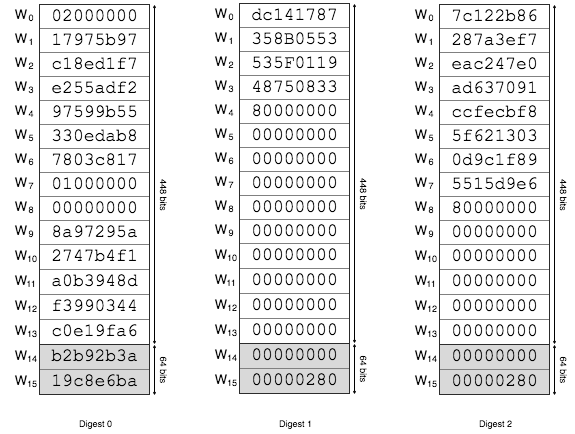
\includegraphics[scale=0.59]{img/Bitcoin_block_SHA_256_W0_W15_x3}
        \caption{Los primeros 16 registros de la variable $W_{t}$ en los tres casos en los que se ha de ejecutar la función SHA-256.}
    \end{figure}

\section{Almacenamiento en ficheros}
    A continuación un ejemplo de los datos de un bloque almacenados en un fichero blk*.dat.
    \begin{figure}[H]
        \centering
            \begin{minted}{c}
00000000  f9 be b4 d9 c5 e2 13 00  00 e0 00 20 17 0f da d7  |........... ....|
00000010  d4 1e 65 f2 62 0b 99 72  f1 0d 1e 22 ee 8d be 1d  |..e.b..r..."....|
00000020  f6 e2 14 00 00 00 00 00  00 00 00 00 f3 82 f9 60  |...............`|
00000030  15 b3 89 58 3a 8a a6 87  ff 19 65 1d 72 98 03 46  |...X:.....e.r..F|
00000040  1b 10 a0 a7 bd 6e 09 68  29 f3 a5 6f 63 b2 6d 5c  |.....n.h)..oc.m\|
00000050  88 6f 2e 17 00 17 1b 7f  fd 58 0c 01 00 00 00 00  |.o.......X......|
00000060  01 01 00 00 00 00 00 00  00 00 00 00 00 00 00 00  |................|
00000070  00 00 00 00 00 00 00 00  00 00 00 00 00 00 00 00  |................|
00000080  00 00 ff ff ff ff 4d 03  dc 9a 08 04 3d b2 6d 5c  |......M.....=.m\|
00000090  2f 70 6f 6f 6c 69 6e 2e  63 6f 6d 2f fa be 6d 6d  |/poolin.com/..mm|
000000a0  d6 c3 c4 23 3d 5d ea ad  18 de cc 86 2c 97 c0 7f  |...#=]......,...|
000000b0  d4 9f 3e da 2c a4 54 b1  b6 16 bd 40 f5 cb 6b 47  |..>.,.T....@..kG|
000000c0  01 00 00 00 00 00 00 00  d5 27 bc 06 6b 58 00 00  |.........'..kX..|
000000d0  00 00 00 00 ff ff ff ff  02 ff a0 73 4d 00 00 00  |...........sM...|
000000e0  00 17 a9 14 b7 57 c3 e4  65 37 06 dd 01 f7 b8 34  |.....W..e7.....4|
000000f0  5a 6d 71 d9 6a 7b 13 6b  87 00 00 00 00 00 00 00  |Zmq.j{.k........|
00000100  00 26 6a 24 aa 21 a9 ed  e7 29 55 44 b2 a5 b2 1e  |.&j$.!...)UD....|
00000110  72 27 71 3f 65 d5 7c ec  e8 e2 1a 1a c7 90 c3 ee  |r'q?e.|.........|
00000120  a4 fe 43 cb 99 6f 55 eb  01 20 00 00              |..C..oU.. ..|
            \end{minted}
        \end{figure}

\end{document}
